\documentclass{beamer}
\usetheme{metropolis}
\usepackage{listings}
\usepackage{xcolor}

\title{Fast data structures and APIs}
\author{Jannusch Bigge}
\date{19.12.2023}

\begin{document}
\begin{frame}
    \titlepage
\end{frame}

\section{Fast data structures}

\begin{frame}{Fast data structures}
    By now you should know the following data structures:
    \begin{itemize}
        \item Lists
        \item Tuples
        \item Sets
        \item Dictionaries
    \end{itemize}
    \pause
    These are all handy, but sometimes you need something special.
\end{frame}

\section{The Problem}

\begin{frame}{The Problem}
    We have a list of numbers.\pause
    \only<2>{\begin{figure}
        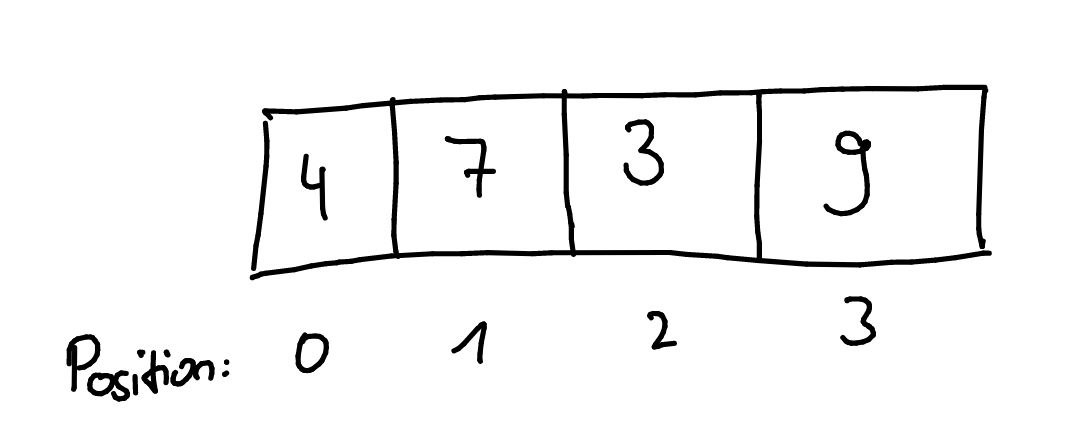
\includegraphics[width=0.8\textwidth]{fig/start.jpg}
    \end{figure}
    }
    \only<3>{\\And we want to add something to the end.\pause\begin{figure}
        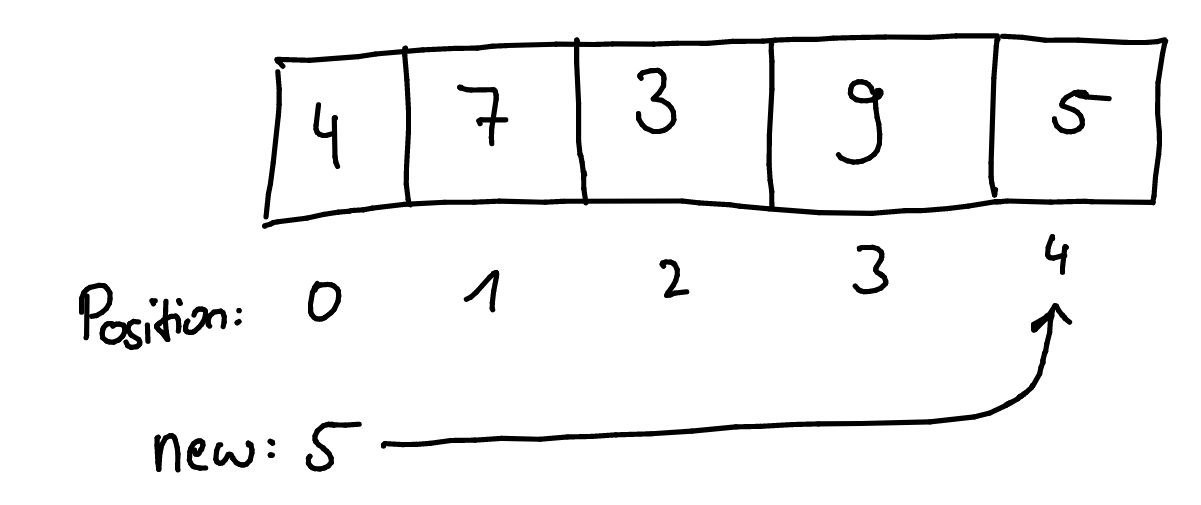
\includegraphics[width=0.8\textwidth]{fig/new_end.jpg}
    \end{figure}}
    \only<4>{\\Now we want to add something to the begin.\pause\begin{figure}
        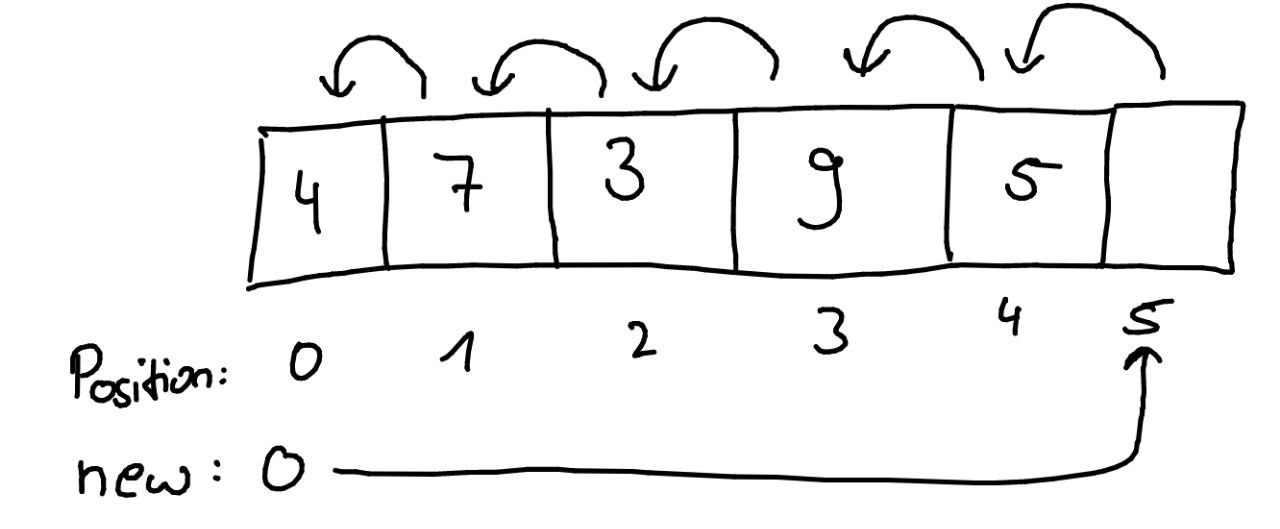
\includegraphics[width=0.8\textwidth]{fig/new_zero.jpg}
    \end{figure}}
    \only<5>{\\With some more numbers now.\pause\begin{figure}
        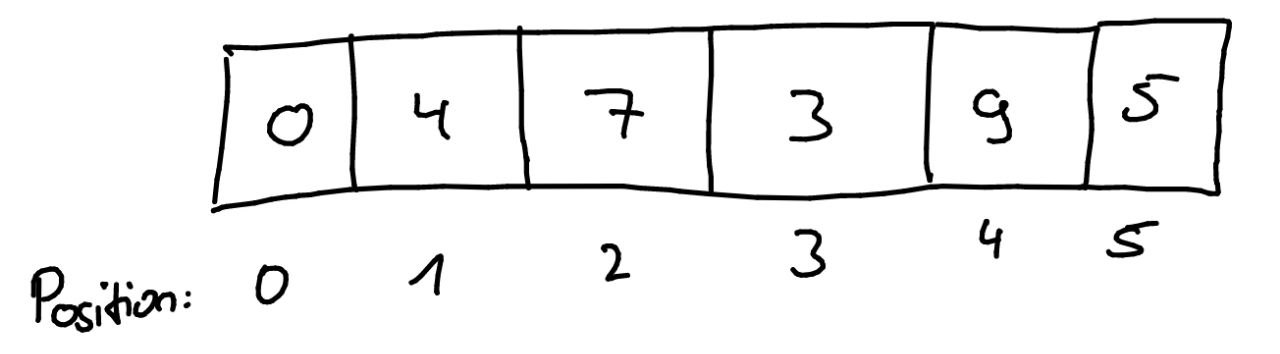
\includegraphics[width=0.8\textwidth]{fig/end.jpg}
    \end{figure}}
\end{frame}

\begin{frame}[fragile]{The Problem}
    \begin{alertblock}<1->{Adding something to the end is easy.}
        \begin{itemize}
            \item<2-> We just add it to the end.
            \item<3-> This takes $O(1)$ time.
        \end{itemize}
    \end{alertblock}
    \begin{alertblock}<4->{Adding something to the begin is hard.}
        \begin{itemize}
            \item<5-> We have to move all the other elements.
            \item<6-> This takes $O(n)$ time.
            \item<7-> pop(0) is the same.
        \end{itemize}
    \end{alertblock}
\end{frame}

\begin{frame}
    Just reverse the list, stupid!
\end{frame}

\begin{frame}{deque}
    There is a data structure that can do both in $O(1)$ time: \textbf{deque}\pause
    \begin{itemize}
        \item It is short for \textbf{double ended queue}.
        \item It is a list that can be appended and prepended in $O(1)$ time.
        \item It is implemented as a doubly linked list.
        \item It is in the \textbf{collections} module.
        \item It is a bit slower than a list.
    \end{itemize}
    
\end{frame}

\begin{frame}[fragile]{deque}
    Some examples:
    \begin{lstlisting}[language=Python, backgroundcolor = \color{lightgray}]
from collections import deque
d = deque(range(1, 5))
d.append(5)     # append to the end
d.appendleft(0) # append to the begin
list(d)         # returns list of deque
d.rotate(1)     # rotate the deque
    \end{lstlisting}
    \end{frame}

    \section{And an other one}

    \begin{frame}{New Problem}
        We have a list of numbers.\pause
        \only<2>{\begin{figure}
            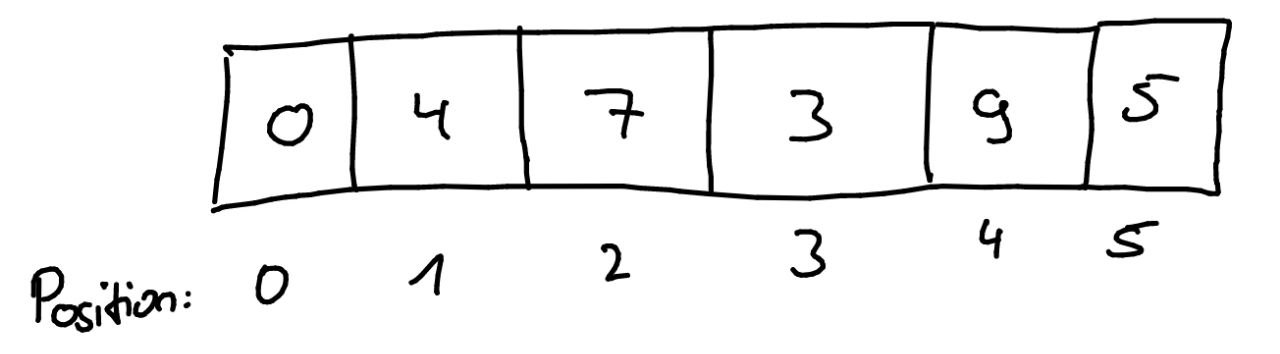
\includegraphics[width=0.8\textwidth]{fig/end.jpg}
        \end{figure}
        }
        \only<3>{\\And we want to find 3.\pause\begin{figure}
            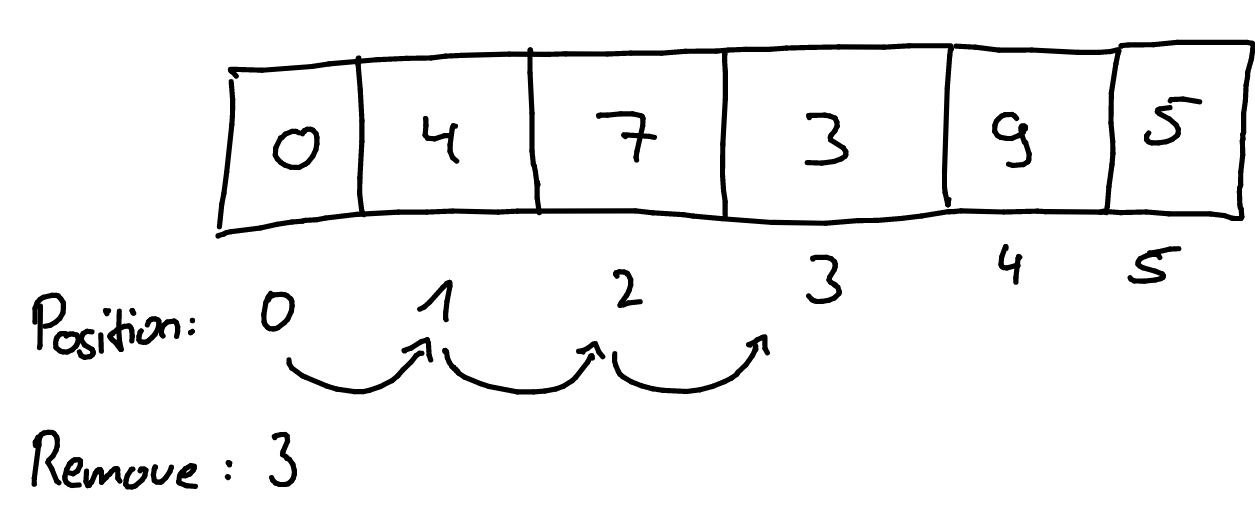
\includegraphics[width=0.8\textwidth]{fig/find_3.jpg}
        \end{figure}}
        \only<4>{\\Now we want to find the max element.\pause\begin{figure}
            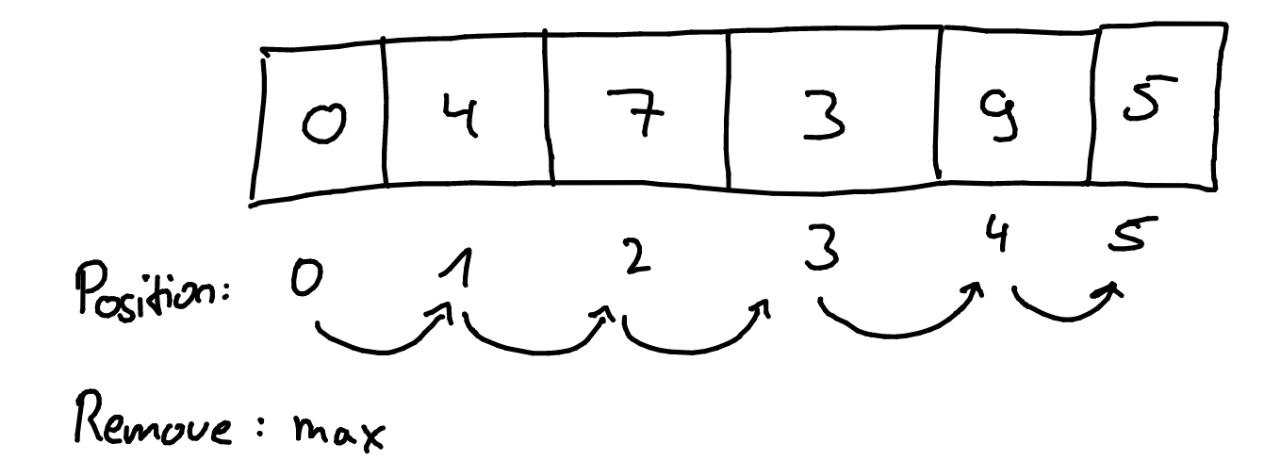
\includegraphics[width=0.8\textwidth]{fig/find_max.jpg}
        \end{figure}}
        \only<5>{\\Now we want to find the max element.\pause\begin{figure}
            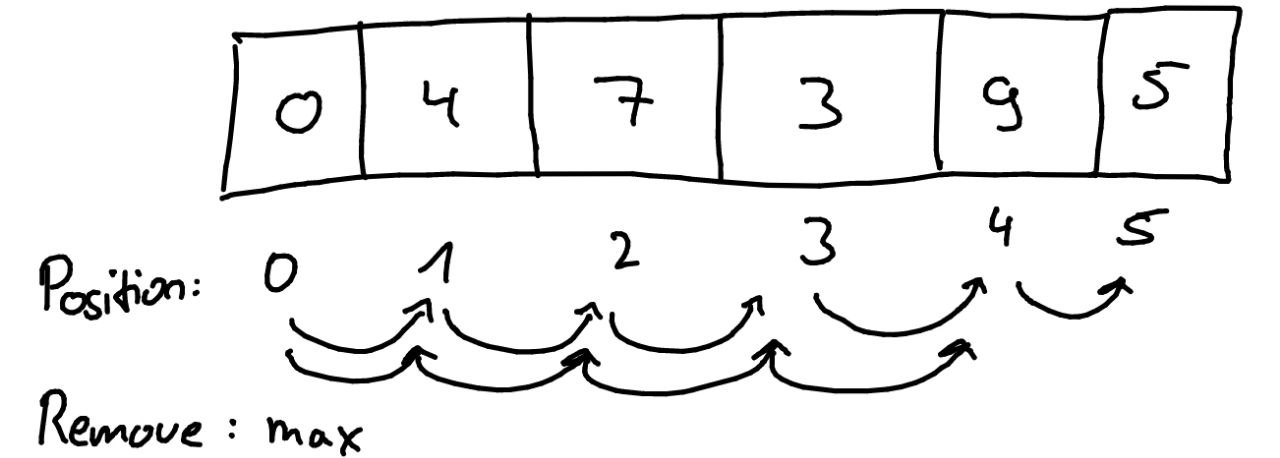
\includegraphics[width=0.8\textwidth]{fig/mid.jpg}
        \end{figure}}
        \only<6>{\\Finaly we have to shrink the list.\pause\begin{figure}
            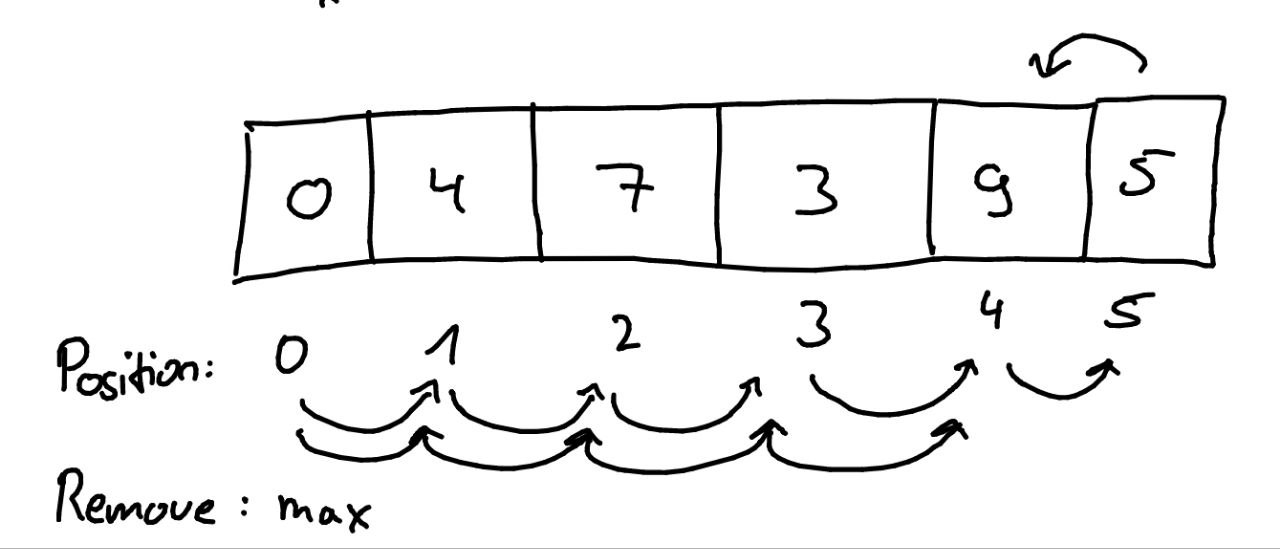
\includegraphics[width=0.8\textwidth]{fig/end_2.jpg}
        \end{figure}}
    \end{frame}

    \begin{frame}{heapqueue}
        There is a data structure that can delete in $O(\log n)$ and find even in $O(1)$ time: \textbf{heapqueue}\pause
        \begin{itemize}
            \item It is a list that can be appended and prepended in $O(\log n)$ time.
            \item It is implemented as a binary heap.
            \item It is in the \textbf{heapq} module.
            \item It is a bit slower than a list.
        \end{itemize}
        
    \end{frame}

    \begin{frame}[fragile]{heapqueue}
        Some examples:
        \begin{lstlisting}[language=Python, backgroundcolor = \color{lightgray}]
from heapq import heappush, heappop, heapify
h = []
heappush(h, 5) # append to the end
heappush(h, 0) # append to the begin
heappop(h)     # pop the smallest element
        \end{lstlisting}
        \end{frame}

        \section{APIs}
        \begin{frame}{REST API}
            We want to get Data from a Website.\pause
            The owner of the site is nice and provides an API.\pause
            \begin{itemize}
                \item We use \textbf{requests} to get the data.
                \item We use \textbf{json} to parse the data.
            \end{itemize}
        \end{frame}

            \begin{frame}[fragile]{REST API}
                Some examples:
                \begin{lstlisting}[language=Python, backgroundcolor = \color{lightgray}]
import requests
import json
r = requests.get('https://api.github.com/events')
r.status_code # returns status code
r.json() # returns json
                \end{lstlisting}
            \end{frame}

                \begin{frame}{What happens here?}
                    The \textbf{requests} module sends a \textbf{GET} request to the server.\pause
                    We have different types of requests:
                    \begin{itemize}
                        \item \textbf{GET} - get data
                        \item \textbf{POST} - send data
                        \item \textbf{PUT} - update data
                        \item \textbf{DELETE} - delete data
                    \end{itemize}
                    This requests are called \textbf{HTTP} requests.
                \end{frame}
                
                \begin{frame}{The response}
                    The server responds with a \textbf{status code} and some \textbf{data}.\\\pause
                    This status codes are common:
                    \begin{itemize}
                        \item \textbf{200} - OK
                        \item \textbf{404} - Not Found
                        \item \textbf{500} - Internal Server Error
                    \end{itemize}
                \end{frame}

                \begin{frame}[fragile]{The response}
                    First we should check the status code:
                    \begin{lstlisting}[language=Python, backgroundcolor = \color{lightgray}]
r = requests.get('https://api.github.com/events')
r.status_code # returns status code
                    \end{lstlisting}
                    \pause
                    Then we can parse the data:
                    \begin{lstlisting}[language=Python, backgroundcolor = \color{lightgray}]
r.text # returns the data (aka text) as string
r.json() # returns a json object of the text
    \end{lstlisting}
                \end{frame}

                \begin{frame}{json}
                    Json is a why to represent data as a string.\pause
                    It is a bit like a dictionary. And therefor there is a module that can parse it.\pause
                    \begin{itemize}
                        \item \textbf{json.loads} - parse a string
                        \item \textbf{json.dumps} - create a string
                    \end{itemize}
                    
                \end{frame}

                    

                \section{Task}
                \begin{frame}{Task}
                    \begin{itemize}
                        \item Read the data of a river
                        \item https://www.pegelonline.wsv.de/webservice/ueberblick
                        \item Create a plot of the water level over time
                    \end{itemize}
                    \end{frame}

\end{document}

